\subsection{Sustitución}
La idea es tomar una parte de una formula y sustituirla por algo equivalente que sea más manejable. Definamos de forma rigurosa el concepto. 

\begin{figure}[h]
\centering
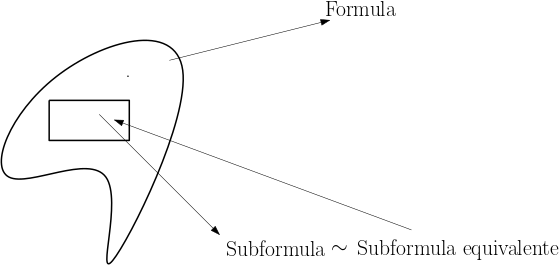
\includegraphics[width=8cm]{susti}
\end{figure}

\begin{definition} Sean $\varphi, \, \psi \in \p$ y $p \in \mbox{SP}$, se denota
\[ \psi[\varphi/p] \]
a sustituir en la fórmula $\psi$ las apariciones de $p$ por $\varphi$. Para definir la sustitución utilizamos el método de recursión. De este modo, obtenemos 
\begin{itemize}
    \item[(AT)] Para las formulas atómicas se tiene que
    \begin{itemize}
    	\item $p[\varphi/p] = \varphi$.
    	\item $q[\varphi/p] = q \quad q \neq p$.
    	\item $\top[\varphi/p] = \top$.
    	\item $\bot[\varphi/p] = \bot$.
    \end{itemize}
    \item[($\neg$)] $(\neg\psi)[\varphi/p] = \neg(\psi[\varphi/p])$.
    \item[($\Box$)] $(\psi_1 \boox \psi_2)[\varphi/p] = (\psi_1[\varphi/p] \boox \psi_2[\varphi/p])$.
\end{itemize}
\end{definition}

De manera esquemática 

\begin{figure}[h]
\centering
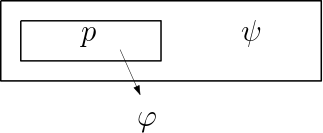
\includegraphics[width=4cm]{esq}
\end{figure}

\begin{theorem}
Sean $\varphi, \varphi', \psi \in \p$, $p \in SP$. Si $\varphi \sim \varphi'$, entonces $\psi[\varphi/p] \sim \psi[\varphi'/p]$.
\end{theorem}

\textbf{Notación}. Dada
\[f:  A  \rightarrow  B\]
se tiene que
\[f[b/a](x)= \left \lbrace \begin{matrix}
f(x) & \mbox{si} & x \neq a\\
b & \mbox{si} & x = a
\end{matrix}\right. \]

\begin{lemma}
Sean $\varphi, \psi \in \p$, $p \in \mbox{SP}$ y $v$ valoración. Entonces:
\[ \widehat{v}(\psi[\varphi/p]) =  v[\widehat{\widehat{v}(\varphi)/p}](\psi)\]
\end{lemma}
\begin{proof}
Procedemos por inducción estructural sobre $\psi$. Comenzamos por las atómicas
\begin{itemize}
\item[(AT)]
\begin{itemize}
	\item Si $\psi = p$ entonces, $\psi[\varphi/p] = \varphi$. Luego 
    	 \[ \widehat{v}(\psi[\varphi/p]) = \widehat{v}(\varphi) \]
   	\item Si $\psi = q$ con $q \neq p$ entonces $\psi[\varphi/p] = q$, con lo que $\widehat{v}(\psi[\varphi/p]) = \widehat{v}(q)$, luego 
   	\[ v[\widehat{\widehat{v}(\varphi)/p}](q) = \widehat{v}(q) \]
   	\item Si $\psi = \top$, $\psi[\varphi/p] = \top$, luego 
   	\[ v[\widehat{\widehat{v}(\varphi)/p}](\top) = v(\top) = V \]
   	\item Si $\psi = \bot$, $\psi[\varphi/p] = \bot$, luego 
   	\[ v[\widehat{\widehat{v}(\varphi)/p}](\bot) = v(\bot) = F \]
\end{itemize} 
\item[($\neg$)] Si $\psi = \neg \psi_1$, entonces $\widehat{v}((\neg\psi_1)[\varphi/p]) = \widehat{v}(\neg(\psi_1[\varphi/p])) = v_{\neg}(\widehat{v}(\psi_1[\varphi/p]))$ por hipótesis de inducción tenemos que
\[  v_{\neg}(v[\widehat{\widehat{v}(\varphi)/p}])(\psi_1) = v[\widehat{\widehat{v}(\varphi)/p}](\neg\psi_1) \]   
\item[($\Box$)] Si $\psi = \psi_1 \boox \psi_2$, entonces 
\[ \widehat{v}(\psi[\varphi/p]) = \widehat{v}((\psi_1[\varphi/p]  \boox  \psi_2[\varphi/p])) = v_{\Box}(\widehat{v}(\psi_1[\varphi/p]), \; \widehat{v}(\psi_2[\varphi/p])) \]
 por hipótesis de inducción  
 \[ v_{\Box}(v[\widehat{\widehat{v}(\varphi)/p}](\psi_1), \; v[\widehat{\widehat{v}(\varphi)/p}](\psi_2)) = v[\widehat{\widehat{v}(\varphi)/p}](\psi_1 \boox \psi_2) \]
\end{itemize}
\end{proof}

\begin{proof}(\textit{Teorema 1}). 
\[ \widehat{v}(\psi[\varphi/p]) = v[\widehat{\widehat{v}(\varphi)/p}](\psi) =_{1} v[\widehat{\widehat{v}(\varphi')/p}](\psi) = \widehat{v}(\psi[\varphi'/p])\]
en (1) utilizamos que $\widehat{v}(\varphi)=\widehat{v}(\varphi')$.
\end{proof}

\addtocounter{ej}{1} % sumo 1
\textbf{Ejemplo \Roman{ej}}: Sean $\varphi=p \rightarrow q$ y $\psi=r \rightarrow t$ y tomamos la sustitución $\psi[\varphi/r]=(p \rightarrow q) \rightarrow t$. Entonces, es indiferente valorar $\psi[\varphi/r]$ en
 
\begin{center}
\begin{tabular}{|c|c|c|c|}
\hline 
\textbf{p} & \textbf{q} & \textbf{r} & \textbf{t} \\ 
\hline 
V & F & V & V \\ 
\hline 
\end{tabular}
\end{center}
 
que valorarlo, siendo $\widehat{v}(\varphi)=F$, entonces $v[\widehat{v}(\varphi)/r]$

\begin{center}
\begin{tabular}{|c|c|c|c|}
\hline 
\textbf{p} & \textbf{q} & \textbf{r} & \textbf{t} \\ 
\hline 
V & F & F & V \\ 
\hline 
\end{tabular} 
\end{center}
\paragraph{}
\begin{lemma}
Si $\psi_1 \sim \psi_2$ entonces $\psi_1[\varphi/p] \sim \psi_2[\varphi/p]$.
\end{lemma}
\begin{proof}
En efecto
\[ \widehat{v}(\psi_1[\varphi/p]) = v[\widehat{\widehat{v}(\varphi)/p}](\psi_1)=\]
como $\psi_1 \sim \psi_2$
\[  v[\widehat{\widehat{v}(\varphi)/p}](\psi_2)=\widehat{v}(\psi_2[\varphi/p]) \]
\end{proof}

\addtocounter{ej}{1} % sumo 1
\textbf{Ejemplo \Roman{ej}}: Si queremos ver $\varphi \wedge \psi \sim \psi \wedge \varphi$ basta tomar $\psi_1= p \wedge \psi$ y $\psi_2= \psi \wedge p$ y aplicar el lema anterior. 
\paragraph{}
\textbf{Observación}. Esto implica que, gracias al lema de sustitución, las leyes de equivalencia vistas en la sección \ref{sec:Leyes de equivalencia logica}, es también aplicable a fórmulas completas. 